\documentclass{article}
%%%%%%%%%%%%%
% Loads packages
%%%%%%%%%%%%%
\usepackage[table]{xcolor}
\usepackage[utf8]{inputenc}
\usepackage[colorlinks=true,linkcolor=blue]{hyperref}
\usepackage{geometry} %package needed to set margins
\usepackage{fancyhdr}
\usepackage{graphicx}
\usepackage{amsmath}
\usepackage{amsthm}
\usepackage{mdframed}
\usepackage{tikz}
\usetikzlibrary{arrows.meta}
\usetikzlibrary{decorations.markings}
\usepackage{amsfonts}
\usepackage{wasysym}

\usepackage{listings}% http://ctan.org/pkg/listings
\lstset{
  basicstyle=\ttfamily,
  mathescape
}


\pagestyle{fancy}
\fancyhf{}
\chead{\textbf{Homework 8}}
\lhead{Math 213, Fall 2024}
\rhead{Due Sunday, 11/3 at 11:59pm}

%%%%%%%%%%%%%
% Sets margins
%%%%%%%%%%%%%
\newgeometry{left=1.5in,right=1in,top=1in,bottom=1in}
\setlength\headsep{3pt}

%%%%%%%%%%%%%
% Creates problem and solution environments
%%%%%%%%%%%%%

% Solution Environment
\newenvironment{solution}{\begin{proof}[Solution]}{\end{proof}}

% Problem Environment
\newenvironment{problem}[1]
    {\begin{mdframed}[default]
    \textbf{Problem #1:}
    }
    {\end{mdframed}
    }
    
%%%%%%%%%%%
% Custom Commands
%%%%%%%%%%%
\newcommand{\gOne}{\cellcolor{green!50!white} 1}
\newcommand{\rZero}{\cellcolor{red!50!white} 0}

\begin{document}


\begin{problem}{\S 8.6 - 3}
How many solutions does the equation $x_1 + x_2 + x_3 = 13$ have where $x_1, x_2,$ and $x_3$ are nonnegative integers less than 6?
\end{problem}

\begin{problem}{\S 8.6 - 10}
In how many ways can eight distinct balls be distributed into three distinct urns if each urn must contain at least one ball?
\end{problem}

\begin{problem}{\S 8.6 - 14}
What is the probability that none of 10 people receives the correct hat if a hatcheck person hands their hats back randomly?
\end{problem}

\begin{problem}{\S 9.1 - 6(a-f)}
Determine whether the relation $R$ on the set of all real number is reflexive, symmetric, antisymmetric, and/or transitive, where $(x,y) \in R$ if and only if
\begin{itemize}
    \item[(a)] $x+y = 0$.
    \item[(b)] $x = \pm y$.
    \item[(c)] $x-y$ is a rational number.
    \item[(d)] $x = 2y$.
    \item[(e)] $xy \geq 0$.
    \item[(f)] $xy = 0$.
\end{itemize}
\end{problem}

\begin{problem}{\S 9.1 - 15}
Can a relation on a set be neither reflexive nor irreflexive?
\end{problem}

\begin{problem}{\S 9.1 - 22}
Must an asymmetric relation also be antisymmetric? Must an antisymmetric relation also be asymmetric?
\end{problem}

\begin{problem}{\S 9.1 - 26}
Let $R$ be the relation $R = \{ (a,b) : a < b \}$ on the set of integers. Find
\begin{itemize}
    \item[(a)] $R^{-1}$.
    \item[(b)] $\overline{R}$.
\end{itemize}
\end{problem}

\begin{problem}{\S 9.3 - 2(a,b)}
Represent each of these relations on $\{ 1, 2, 3, 4 \}$ with a matrix (with the elements of this set listed in increasing order).
\begin{itemize}
    \item[(a)] $\{ (1,2),~(1,3),~(1,4)~,(2,3),~(2,4),~(3,4) \}$
    \item[(b)] $\{ (1,1),~(1,4),~(2,2),~(3,3),~(4,1) \}$
\end{itemize}
\end{problem}

\begin{problem}{\S 9.3 - 14(a-d)}
Let $R_1$ and $R_2$ be relations on a set $A$ represented by the matrices
\begin{align*}
    M_{R_1} = \begin{bmatrix} 0 & 1 & 0 \\ 1 & 1 & 1 \\ 1 & 0 & 0 \end{bmatrix} \qquad \textrm{and} \qquad
    M_{R_2} = \begin{bmatrix} 0 & 1 & 0 \\ 0 & 1 & 1 \\ 1 & 1 & 1 \end{bmatrix}
\end{align*}
Find the matrices that represent
\begin{itemize}
    \item[(a)] $R_1 \cup R_2$.
    \item[(b)] $R_1 \cap R_2$.
    \item[(c)] $R_2 \circ R_1$.
    \item[(d)] $R_1 \circ R_1$.
\end{itemize}
\end{problem}

\begin{problem}{\S 9.3 - 22}
Draw the directed graph that represents the relation \[ \{ (a,a),~(a,b),~(b,c),~(c,b),~(c,d),~(d,a),~(d,b) \}. \]
\end{problem}

\begin{problem}{\S 9.3 - 26}
List the ordered pairs in the relations represented by the directed graph
\begin{center}
    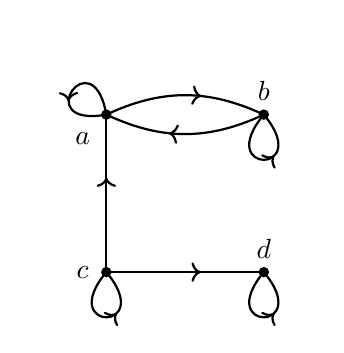
\begin{tikzpicture}
        \begin{scope}[thick,decoration={
            markings,
            mark=at position 0.6 with {\arrow{>}}}
            ] 
        % draw vertices
        \node[circle, fill=black,scale = 0.4] at (0,0){};
        \node[circle, fill=black,scale = 0.4] at (2,0){};
        \node[circle, fill=black,scale = 0.4] at (0,2){};
        \node[circle, fill=black,scale = 0.4] at (2,2){};
        
        % draw directed edges
        \draw[postaction={decorate}] (0,0) to (2,0);
        \draw[postaction={decorate}] (0,0) to (0,2);
        \draw[postaction={decorate},out=25,in=155] (0,2) to (2,2);
        \draw[postaction={decorate},out=205,in=-25] (2,2) to (0,2);
        \draw[scale=2,postaction={decorate}] (0,0) to[out=-130,in=-50,loop] (0,0);
        \draw[scale=2,postaction={decorate}] (0,1) to[out=100, in=190,loop] (0,1);
        \draw[scale=2,postaction={decorate}] (1,0) to[out=-130,in=-50,loop] (1,0);
        \draw[scale=2,postaction={decorate}] (1,1) to[out=-130,in=-50,loop] (1,1);
        
        % labels vertices
        \node at (-0.3,0) {$c$};
        \node at (2,0.3) {$d$};
        \node at (-0.3,1.7) {$a$};
        \node at (2,2.3) {$b$};
        \end{scope}
    \end{tikzpicture}
\end{center}
\end{problem}


\end{document}